\documentclass{imc-inf}
\usepackage{graphicx}

\title{Implementation and analysis of a machine learning approach to long-term values investing}
\subtitle{Minimize risk while maximizing cash flow through stock picking based on fundamental company data}
\thesistype{Bachelor Expos\'e} % or Bachelor Expos\'e
\author{Daniel Netzl}
\supervisor{Dr. Rubén Ruiz Torrubiano}
\copyrightyear{2021}
\submissiondate{19.04.2023}
\keywords {Data Analytics, Machine Learning, Stock Market, Value Investing, Data Mining, Deep Learning, Defensive Investing, Data Science, Random Forest, Neural Network} % add keywords here 



% \usepackage{xyz}
% ... add your own packages here!
\usepackage{listings}
\usepackage{subcaption}
                              

\begin{document}
\frontmatter\maketitle{}


\begin{declarations}\end{declarations}


\addtoToC{Table of Contents}%
\tableofcontents%
\clearpage


\addtoToC{List of Tables}%
\listoftables
\clearpage


\addtoToC{List of Figures}%
\listoffigures
\clearpage


%   MAIN MATTER  %%%%%%%%%%%%%%%%%%%%%%%%%%%%%%%%%%%%%%%%%%%%%%%%%%%%%%%%%%%%%%
\mainmatter%

\chapter{Introduction}\label{chap:introduction}

\section{Motivation}%\label{chap:motivation}
When it comes to investing in the financial market, there are numerous approaches and tactics to consider. Investors strive for long-term success, but they frequently fail for a variety of reasons. Younger investors, in particular, have a tendency to underestimate the risk and end up accepting a significant financial loss. That has been more common in recent years, with a significant portion of generation Z following self-proclaimed “gurus” and their “expert” opinions and recommendations on numerous internet platforms. Following those incoherent investing schemes is tantamount to speculation or outright gambling. The promise of quick and cheap returns attracts investors, who fall prey to Wall Street's countless fads. In this paper, the author has two objectives. The first half of the paper describes the common mistakes made by investors and the challenges they confront, particularly in the present era of easy access to financial markets. In the second half of the paper the author provides his approach to asset management, as well as an algorithm that may aid him in executing it, in the hopes of assisting investors in recognizing and so avoiding these losing methods ~\cite{margin_of_safety}.

The author will advocate one specific investing technique for the remainder of the paper: the value-investment philosophy. This idea encapsulates the technique of investing in assets that trade at a significant discount to their intrinsic value. The strategy has been used for a long time, with investors experiencing minimal risk and good rewards ~\cite{margin_of_safety}.
To achieve investment success, it is of utmost importance to know where others go wrong and deliberately choose a path to avoid those pitfalls. The thesis will mainly be built upon the most honorable representatives of value investing, including Benjamin Graham, David Dodd, and Seth Klarman. 

Security Analysis ~\cite{security_analysis}, written by Benjamin Graham and David Dodd more than fifty years ago, is widely considered as the bible of value investing. For generations of value investors, that single work has paved the road. Graham's most recent book, The Intelligent Investor ~\cite{the_intelligent_investor}, is a less scholarly account of the value-investing process. Warren Buffett, the chairman of Berkshire Hathaway, Inc., and a Graham student, is widely recognized as the most successful value investor today ~\cite{margin_of_safety} Seth Klarman published the most recent book this thesis’ methods are based on. With Margin of Safety ~\cite{margin_of_safety} Klarman emphasizes the necessity of avoiding typical blunders. By describing his approach to value investing, he demonstrates that success in the financial markets requires a defined strategy backed by patience, ambition, and hard effort.

\section{Problem Definition}%\label{chap:problem defintion}
It's terrifying to see how many naïve and ingenious investors have had horrible financial outcomes. If this paper and its algorithm succeed in their approach, the author will be overjoyed if he can persuade even a few of the readers to avoid risky investment selections in favor of sensible ones that will safeguard and keep their hard-earned cash.
Investors are frequently their own worst adversaries. On the one hand, when price trends are rising, investors are more likely to speculate and follow their emotional greed, placing high-risk bets based on optimistic expectations and ignoring related danger. When prices are declining, on the other hand, emotions again play a huge role. Fear of loss causes the investors to concentrate solely on the prices continuing to fall, rather than on the underlying data of the companies. Regardless of the current market scenario, many people are looking for a winning recipe. Reality, however, does not follow any mathematical equations.

Younger investors, in particular, are more likely to acquire their financial advice from dubious sources, such as influencers who claim to have had amazing success on Wall Street and know exactly what they are doing. Due to the ease of access to financial markets and the availability of super-cheap transactions provided by online brokers, a significant portion of Generation Z is perceived to be significantly involved in extremely speculative high-frequency trades. 
This effect has been particularly noticeable in recent years, when market prices have only shown one direction. The S\&P 500, for example, climbed by over 98 percent between May 2017 and January 2022. That's nearly a 20 percent annual increase. The NASDAQ 100 hit its interim peak around the same time, gaining roughly 190 percent, or 38 percent annually, in the same time frame. It goes without saying that many new investors were enticed by the supposedly easy and extraordinary gains.
However, as this paper is written, those new investors are experiencing their first baisse, revealing their expertise to be nothing more than riding a wave together with the rest of the market. It is critical to understand what one is doing and to have a clear approach during such times.

The strength of such speculative investors should not be underestimated. As can be observed in the case of the Gamestop stock, a downward-pointing company's stock price has risen by over a thousand percent in half a year, only to plummet by half immediately after (but still remain at a high level). There have been multiple instances where private investors have banded together on social media, particularly on the website reddit.com, to artificially inflate prices to unheard-of highs, enticing a large number of naive investors and leaving the vast majority of them with irreversible losses. Many individual and institutional investors overlook or deliberately disregard core corporate principles, perceiving stocks as nothing more than pieces of paper to be traded back and forth.

Investors must ultimately choose their preferred methods. Either they take a seemingly simple way that provides the comfort of consensus, or they take a path that involves emotional responses fueled by greed and fear and guided by short-term thinking ~\cite{margin_of_safety}.

Most people are unwilling to make the commitment required by the alternative. Those methods, which include value investing, involve fundamental analysis, which treats equities as fractional ownership of the underlying company they represent ~\cite{margin_of_safety}.

It is critical to distinguish between speculation and investing. Anyone who buys and sells stocks nowadays is referred to be an investor. Nonetheless, the vast majority makes no attempt to justify their investing decision. Most of the time, no evaluations are performed, and stocks are bought and sold when markets rise and fall. The recent trend of the stock price is frequently used as a buying criterion. If the stock outperformed the market, it gets purchased. If any analysis is conducted, they frequently include a review of long-term past growth that is expected to continue. Also, "investors" may select companies that have not yet produced spectacular outcomes but are expected to do so in the future. Growth stocks and assets from the technological or health-care sectors are common in these companies. "Investors" hope to benefit from enormous future results ~\cite{the_intelligent_investor}. 

The "investor" faces two distinct dangers in his search for the most promising stocks. He or she could be wrong about the company's future progress. Even if he is correct, the present market price may already reflect the anticipated development. Insofar as they are predictable, a company's near-future results are often already taken into account. By making a judgment based on those criteria, one is likely to discover that others have already done so. To summarize, in order to obtain above-average results, one must adhere to policies that are essentially sound and promising, even if they are unpopular on Wall Street ~\cite{the_intelligent_investor}.
Value investing aims to identify stocks that have been overlooked and are consequently undervalued. However, it is not so straightforward, since the process requires a lot of patience. Selling an overrated and overly popular issue takes boldness and endurance. The theory is sound, and while successful application is not impossible, mastering it is a difficult art ~\cite{the_intelligent_investor}. Even more so nowadays when stock prices are adopted in a fraction of a second.

Even yet, the concept of value investing is unlikely to turn anyone into a profitable value investor. Hard work and tight discipline are required for value investment. Only a small percentage of people are willing and able to devote the necessary time and effort, and only a small percentage of people have the right mindset to be successful in the long run. Because those virtues are becoming increasingly rare as the modern environment becomes more dynamic, the algorithm under investigation tries to aid in making value investing accessible to a wider audience.

Naturally, this paper will not present a foolproof investment method. It will not guarantee any profits in advance, but it will highlight the personal risk that everyone must analyze before making investing decisions. The presented theory, as well as the algorithm developed, do not offer any financial advice or suggestions. The algorithm's signals are nothing more than the results of various calculations that, according to the inventor, might be utilized to aid in the discovery of undervalued companies. It is entirely up to the readers to decide how they will use the material.

\section{Research Objectives and Questions}%\label{goal}
The purpose of this bachelor's thesis is to create an algorithm that aids in the making of sound financial decisions. When a selection outperforms its benchmark, the Vanguard FTSE All-World High Dividend Yield Index, in the long run, it is regarded good. During the implementation phase, the author will look for ways to automate the above-mentioned value investing investment technique. The algorithm's foundation will be fundamental company data and its result will be one of three signals: "Buy," "Hold," or "Sell." Please keep in mind that the algorithm only sends out signals based on the data it receives and the machine learning model that was trained on that data. The final product is not a professional investment advice.
The thesis will be regarded successful if the algorithm can consistently exceed its benchmark. The author will see the Efficient Market Theorem refuted in this scenario.

If the target is not accomplished, the author will adhere to the passive investment technique and invest in index funds on a regular basis. In this sense, the author accepts average returns and is unable to disprove the Efficient Market Theorem.

On the road to developing the algorithm the author will examine appropriate machine learning approaches for creating the basis for value investing. Additionally, important features needed for the prediction of the intrinsic value of a company will be determined. This way the author hopes to uncover undervalued companies whose stock prices will increase to a higher extent than the benchmark index.

The machine learning model will utilize backpropagation on historical data to update weights on various features in order to determine the importance of each for predicting the intrinsic value.

It is critical that the model works well over a long period of time, i.e., continuously throughout several years. Short-term success is typically based on luck and cannot be replicated. Technical analysis for speculative short-term stock movement predictions will not be covered in the thesis. The model's results will be assessed on a yearly basis.
The above-mentioned problem statement and goals allow the formulation of the following research questions:

\begin{itemize}
	\item Can a machine learning model based on qualitative and quantitative fundamental company data reliably and accurately predict the intrinsic value of a company?
\end{itemize}

During the implementation, a list of predetermined stocks will be tracked in order to answer the first research question. Each company's qualitative and quantitative data are collected in the hopes of identifying aspects that have a significant impact on the stocks intrinsic worth. A machine learning model is trained for this process. After taking into account a margin of safety, the model compares the stock's suggested price to the current price and issue a "Buy," "Hold," or "Sell" signal.

\begin{itemize}
	\item Can the identified undervalued stocks be used to consistently beat the market and thus disprove the efficient market theorem?
\end{itemize}

The second phase of the empirical study seeks to beat the market using the model's output. To do so, the identified undervalued stocks, i.e., stocks that emit a "Buy" signal, are purchased at a specific moment in the past. The stock picks are evaluated, and their returns are compared to the benchmark index after each of the next ten years.

From those research questions the following hypotheses can be derived:

\begin{itemize}
	\item H0: A machine learning model based on qualitative and quantitative fundamental company data cannot reliably and accurately predict the intrinsic value of a company.
	\item H0: The identified undervalued stocks cannot be used to consistently beat the market and thus the author cannot disprove the efficient market theorem.
	\item H1: A machine learning model based on qualitative and quantitative fundamental company data can reliably and accurately predict the intrinsic value of a company.
	\item H1: The identified undervalued stocks can be used to consistently beat the market and thus the efficient market theorem can be disproved.
\end{itemize}


The following risks are anticipated throughout the thesis:

\begin{itemize}
	\item What qualitative measures should be used to calculate intrinsic value? And how can they be retrieved in bulk?
	\item How can a machine learning technology be used to uncover patterns of undervalued stocks?
	\item How to appropriately assess the model's success within a given time frame and update the model accordingly?
\end{itemize}

\section{Research Methods}

The author's research methodologies are briefly detailed in the next section. These include the data gathering process, the programming language(s) utilized, an implementation plan, a description of the trained machine learning models employed, and an evaluation strategy.

\subsection{Data}%which companies, which data, where to get it from
One of the most crucial questions is for which companies the model makes predictions. Because the value investing method only considers stable companies with a good business model, consistent returns, and low volatility, the focus will be on about 300 companies that have been in the market for a long time and have a history of dividend payouts. Being able to pay dividends on a consistent basis, and even increasing payments in most years, is seen as additional evidence of stability. Still, one should not be fooled by a company's payout ratio, as a high payout and continual dividend increase could be a ruse to appease shareholders.

In a Microsoft Excel file, all the companies are listed with their ticker symbol. This file will be used to access extra data from various online APIs. YahooFinance and Finviz.com are two of the sites that will be used to retrieve financial statement data. Additional web services will be researched to discover if any trustworthy qualitative data sources exist. Automatically retrieving bulk qualitative company data might be a challenge, though. 

The author purposefully includes a huge number of variables from the balance sheet, income statement, and cash flow statement in the prediction models without applying any economic logic to the selection. This allows the models to learn from the data over the whole available time frame which factors and variable combinations perform best for predicting the intrinsic value around earnings announcements over a one-year period.

\subsection{Implementation Plan}%figure which shows the pipeline of the whole process

\begin{figure}[h]
	\centering
	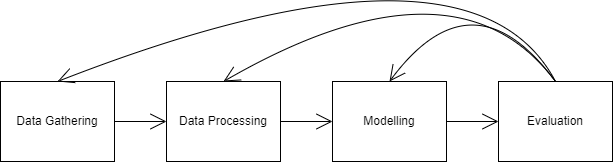
\includegraphics[width=1.0\textwidth]{resources/pipeline.drawio}
	\caption{Implementation plan}
	\label{fig:pipeline}
\end{figure}


\subsection{Machine Learning Models}%figure which explains the model in detail
The machine learning algorithms used in the study include a variety of models that have become increasingly popular in recent years. A Neural Network and a Random Forest model for regression are among them. To benchmark these two models, simpler linear models are used. These include an Ordinary Least Square (OLS) and a Least Absolute Shrinkage and Selection Operator (Lasso) linear regression. As all the models require some dependent variable $y$, the author will make use of two different approaches. 

First, static equations will be employed to determine a company's fair worth using multiple ways. Following that, the dependent variable $y$ will be the average of all the outputs. Those equations include the Discounted Cashflow (DCF) technique, the Graham Stock Valuation Formula (short: Graham Formula), and the Earnings Power Value formula (EPV).

The other approach will involve a self-created program which will label the data entries automatically based on the development of the stock prize a year after. If the stock rose higher than the benchmark, the label will be “Buy”. If the price rose significantly less, whereas different thresholds will be tried out, or even decreased over the period of one year, the label will be “Sell”. Everything in between will be labeled as “Hold”. These labels will be used to validate the output of the machine learning algorithm.


Explain DCF, Graham Formula, EPV

Explain Neural Network

\begin{figure}[h]
	\centering
	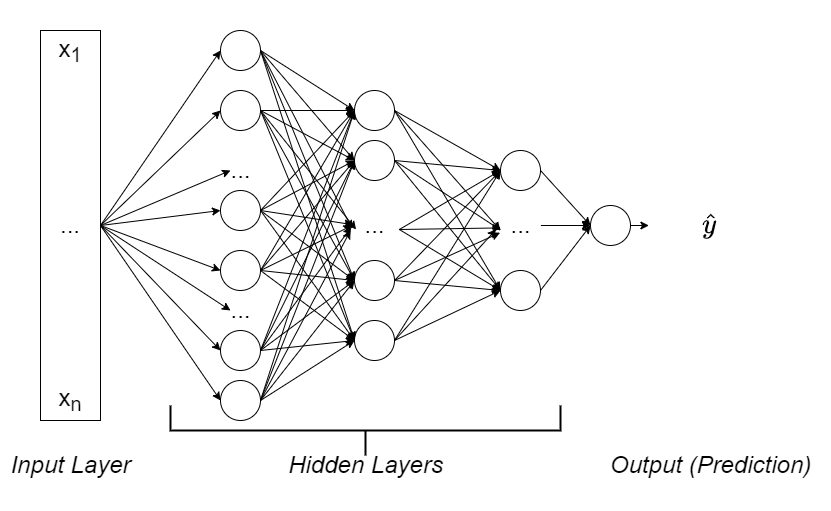
\includegraphics[width=1.0\textwidth]{resources/neural network architecture.png}
	\caption{Neural Network Architecture}
	\label{fig:neural_network}
\end{figure}

Explain Random Forest

\subsection{Training and Test Set}
The training set will contain the quantitative and qualitative fundamental data of each company at the end of each year. This way the time dimension is deliberately left out as (1) that simplifies the models and (2) there is nothing worth remembering from the past. The models analyze current data only and try to estimate a stock’s fair price.  For training purposes 90 percent of the available data will be used, while the remaining 10 percent are used to test the models. 


\subsection{Evaluation Plan}%figure which shows a graph comparing benchmark and a selected stock
A one-year sliding window is used to create the training and test sample for our models. This pane navigates through all the companies in our sample period's records history. Let $P_{t}$ be the price of an issue at any point in time when the algorithm issues a "Buy" signal. Then $P_{t+1}$ represents the price after one year of holding the paper, emulating the purchase of a stock. By subtracting $P_{t}$ from $P_{t+1}$, the return $R_{s,t}$, denoting the return of the individual stock at time $t$, is determined. The result is in continuation compared to the return $R_{i,t}$ of the benchmark index in that exact same time frame. If $R_{s,t_{1}}$ > $R_{i,t_{1}}$ the prediction is considered successful for $t_{1}$. Returns are evaluated until $t_{n}$, where $n$ signifies the last possible complete, i.e., the most recent time frame. The sliding window continues for every year thereafter and after each year, and in total after $t_{n}$, the returns are compared. Once the stock's signal switches to "Sell," the algorithm will cease predicting and calculate $R_{s,t}$ and $R_{i,t}$ to complete the evaluation early.


\section{Code and syntax highlighting}

You may sometimes want to add code snippets to your thesis. You can do so by using \texttt{lstlisting}. Use this with care, as code should not be extensively presented in the thesis. Here is an example. 

\begin{lstlisting}[language=Python]
def addition ():
    print("I am adding numbers here!")
    n = float(input("Enter the number: "))
    t = 0 // Total number enter
    ans = 0
    while n != 0:
        ans = ans + n
        t+=1
        n = float(input("Enter another number (0 to end): "))
    return [ans,t]
\end{lstlisting}

\section{Labels and References}
See \autoref{chap:introduction} for interesting stuff and see a cool logo in \autoref{fig:logo}. If you are still not convinced, try adding a footnote\footnote{did you like it?}. Its easy to add citations, just use a bibtex file to list your references and cite them here like this~\cite{988366}. If you want to read a cool paper~\cite{DBLP:conf/euromicro/DhunganaHW20}, just contact the author of the paper. Haha, that was funny! 


\section{Mathematical Equations and Expressions}
Basic equations in  \LaTeX{} can be easily "programmed". Fermat's Last Theorem (sometimes called Fermat's conjecture, especially in older texts) states that no three positive integers a, b, and c satisfy the equation \[ a^n + b^n = c^n \] for any integer value of $n$ greater than $2$. The cases $n = 1$ and  $n = 1$  have been known since antiquity to have infinitely many solutions. And because its so much fun, here is an integral for you - thank me later!  

\[ \int\limits_0^1 x^2 + y^2 \ dx \]

Do you want a more complex formula, I have no idea what it means, but it looks pretty. 

\[\oint_{i=1}^n \sum_{i=1}^{\infty} \frac{1}{n^s} 
= \prod_p \frac{1}{1 - p^{-s}} \]


\section{Enumerations and Descriptions}
Here is a simple list: 
\begin{enumerate}
	\item The labels consists of sequential numbers.
	\item The numbers starts at 1 with every call to the enumerate environment.
\end{enumerate}

Here is another list: 

\begin{enumerate}
	\item The labels consists of sequential numbers.
	\begin{itemize}
		\item The individual entries are indicated with a black dot, a so-called bullet.
		\item The text in the entries may be of any length.
	\end{itemize}
	\item The numbers starts at 1 with every call to the enumerate environment.
\end{enumerate}

Maybe such descriptions are also useful. These look neat to me. What do you think? Oh, I forgot, this document is not a tutorial. 
\begin{description}
	\item[Short] This is a shorter item label, and some text that talks
	about it. The text is wrapped into a paragraph, with successive
	lines indented.
	\item[Rather longer label] This is a longer item label.  As you can
	see, the text is not started a specified distance in -- unlike
	with other lists -- but is spaced a fixed distance from the end
	of the label.
\end{description}



\section{Adding images}
Adding a simple image is easy. Adding complex images is also easy. What is a complex image anyway? 
\begin{figure}[h]
	\centering
	
\includegraphics[width=1.0\textwidth]{imclogo.png}
	\caption{IMC Logo}
	\label{fig:logo}
\end{figure}





\begin{figure}[ht]
	\begin{subfigure}{.5\textwidth}
		\centering
		% include first image
		
\includegraphics[width=.8\linewidth]{imclogo.png}  
		\caption{Put your sub-caption here}
		\label{fig:sub-first}
	\end{subfigure}
	\begin{subfigure}{.5\textwidth}
		\centering
		% include second image
		
\includegraphics[width=.8\linewidth]{imclogo.png}  
		\caption{Put your sub-caption here}
		\label{fig:sub-second}
	\end{subfigure}
	\caption{Including sub images! }
	\label{fig:fig}
\end{figure}

\section{Tables}

\begin{table}[ht]
\begin{tabular}{ |p{3cm}||p{3cm}|p{3cm}|p{3cm}|  }
	\hline
	\multicolumn{4}{|c|}{Country List} \\
	\hline
	Country Name     or Area Name& ISO ALPHA 2 Code &ISO ALPHA 3 Code&ISO numeric Code\\
	\hline
	Afghanistan   & AF    &AFG&   004\\
	Aland Islands&   AX  & ALA   &248\\
	Albania &AL & ALB&  008\\
	Algeria    &DZ & DZA&  012\\
	American Samoa&   AS  & ASM&016\\
	Andorra& AD  & AND   &020\\
	Angola& AO  & AGO&024\\
	\hline
\end{tabular}
\caption{\label{tab:table-name}Example table}
\end{table}




%   BACK MATTER  %%%%%%%%%%%%%%%%%%%%%%%%%%%%%%%%%%%%%%%%%%%%%%%%%%%%%%%%%%%%%%
%
%   References and appendices. Appendices come after the bibliography and
%   should be in the order that they are referred to in the text.
%
%   If you include figures, etc. in an appendix, be sure to use
%
%       \caption[]{...}
%
%   to make sure they are not listed in the List of Figures.
%

\backmatter%
	\addtoToC{Bibliography}
	\bibliographystyle{IEEEtran}
	\bibliography{references}
	

\begin{appendices} % optional
\chapter{Example Appendix 1}

Appendices should be used for supplemental information that does not form part of the main research. Remember that figures and tables in appendices should not be listed in the List of Figures or List of Tables. 

\chapter{Example Appendix 2}

Appendices should be used for supplemental information that does not form part of the main research. Remember that figures and tables in appendices should not be listed in the List of Figures or List of Tables. 
	
\end{appendices}
\end{document}
